% \subsection{Introduction}

% Image guided radiotherapy (IGRT) is the state-of-the-art tool for reducing patient positioning errors during cancer treatment with radiation\cite{Bujold2012Image-GuidedOutcomes}. When designing a radiotherapy treatment plan, a number of margins around the visible tumors are added to the tumor volume. The final planning tumor volume (PTV) accounts for, among other things, difference in patient positioning during the treatment planning CT scan and during treatment delivered with a linear accelerator. This is generally minimized using IGRT where patient positioning is verified and adjusted based on a  cone beam CT (CBCT) scan acquired on the linear accelerator just prior to treatment. CBCT image quality leads to better alignment, which in turn can lead to tighter PTV margins and increased normal tissue sparing. 

% IGRT is generally performed with kilovoltage (kV) x-ray on-board imagers (OBIs) mounted on the gantry of the linear accelerator at 90 degrees with respect to the megavoltage (MV) treatment beam. OBIs take advantage of the higher image contrast produced by kV CBCT \cite{Alaei2015ImagingTherapy}. However, an alternative approach is to use the megavoltage (MV) treatment beam for image guidance with the aid of an electronic portal imager (EPID). Benefits of this approach include high atomic number artifact reduction\cite{Lindsay2019InvestigationDetector}, less complex linear accelerators without the OBI equipment, and the availability of EPID dosimetry \cite{Mijnheer2013InRadiotherapy,Celi2016EPIDResults}. Limits of this approach include the aforementioned reduction in image contrast compared to kV CBCT due to smaller variation between tissue attenuation coefficients in the MV range, as well as reduced detector quantum efficiency (DQE) due to the more penetrating MV beam. There have been extensive efforts to reduce these limitations.

% To improve MV imaging quality, novel low atomic number (Z) beam targets have been examined to generate photon beams with higher fluence in the kV range. The use of aluminum and carbon targets has been shown to improve image quality: Simulation studies show a 16-19\% increase in contrast between an aluminum target and the default tungsten target for a 6 MV photon beam \cite{Kim2018InvestigationSimulation, Flampouri2002OptimizationExperiment}. Experimentally, Baek et al. showed that a gantry mounted aluminum target improved the limiting spatial frequency (f50) from 0.451 lp/mm to 0.745 lp/mm for a tungsten target  6 MV beam\cite{Baek2019AssessmentFilter}. Additionally, Parsons et al. showed an increase in the contrast to noise ratio (CNR) in projection images of cortical bone by factors ranging from 3.7 to 7.4 between carbon and aluminum targets with 2.35 and 1.9 MV photon beams and the default 6 MV tungsten imaging setup \cite{Parsons2012BeamTargets}.

\begin{figure*}[ht!]
  \begin{center}
%   \captionsetup{justification=centering}
   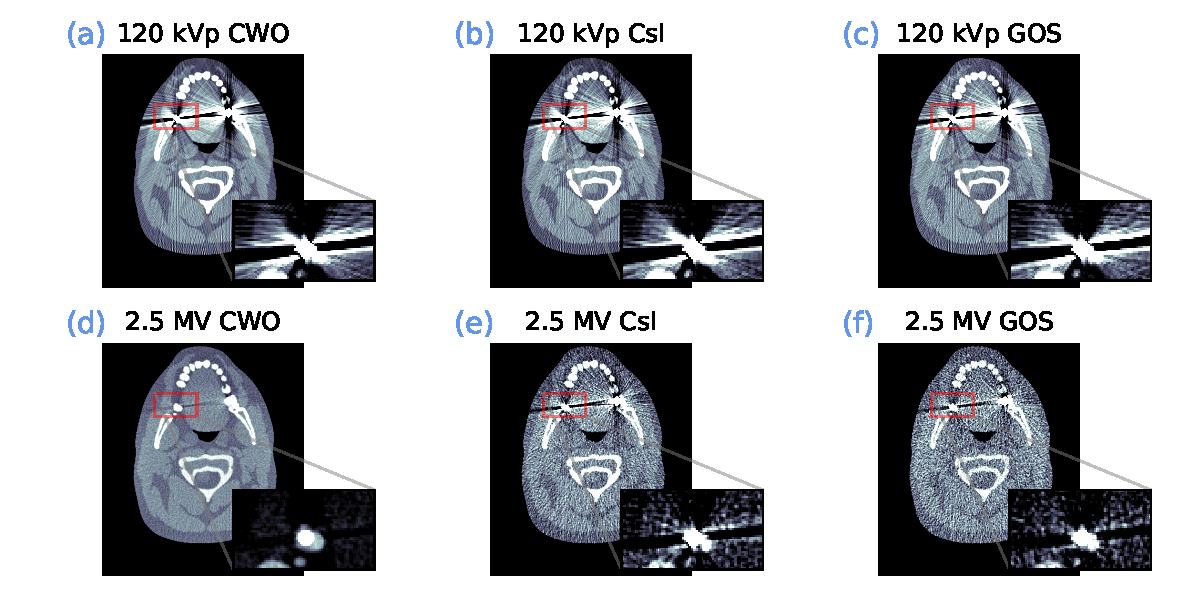
\includegraphics[width=\linewidth,trim={3cm 4cm 2.8cm 4cm}, clip]{figures/Figure_5.pdf}
   \caption{An overview of the simulation setup. a) The phantoms used in this work, the contrast phantom (top) and an XCAT head phantom with silver amalgam fillings (bottom, not all tissues shown in legend). b) The simulation geometry. c) The kV and MV energy spectra.\label{fig_setup_cwo}}
       %note label inside caption
    \end{center}
\end{figure*}

% Furthermore, advances in MV EPID design have shown promise in improving MV image quality. Many MV EPIDs use a gadolinium oxysulfide (GOS) scintillator, which is opaque to its own scintillation photons. This limits the thickness of GOS detectors which in turn limits the quantum efficiency of the detector. Star-lack \textit{et al.} examined cadmium tungstate (CWO) and bismuth germinate (BGO) detectors, which are higher Z materials and can be made thicker for MV photon detection. CWO was noted to have a 20-fold efficiency improvement over GOS with significantly higher stability and light yield than BGO \cite{Star-Lack2015AImaging}. Likewise, image quality improvement was seen using multi-layer GOS imagers with 2-4 times greater CNR than an equivalent single layer GOS detector \cite{Myronakis2020Low-doseMLI}.

% Currently, these two approaches to improving MV imaging, the amelioration of detector efficiencies and introduction of low-Z targets, have remained largely separate. Likewise, direct comparison of the benefit of different imaging strategies in the literature remains challenging as different works have different combinations of voxel size, cone-beam size, phantom dose, focal-spot size and other imaging variables.

% In this work we simulate image quality for combinations of novel MV beam target materials such as carbon and aluminum with different detector materials such as CWO. We compare these novel imaging methodologies with a standard kV imaging setup using a columnar cesium iodide (CsI) detector. We investigate whether the combination of novel MV beams and detectors can result in MV CBCT image quality approaching kV CBCT image quality.

\subsection{Materials and Methods}

% \subsubsection{Experimental Validation}

% (Left) FastCAT was validated against two CBCT images acquired with a Varian Truebeam linac; one using the 100 kVp on board imager with a CsI detector and another using a 6 MV therapy beam with a GOS detector. (Center-right) HU values are compared between the two sets of images for each insert as a function of electron density. All Fastcat HU values showed agreement within the 99\% confidence interval of experimental values. (Right) Detector MTF comparisons to previous works displaying agreement within 5\%.

% \subsubsection{Fastcat}

% The Fastcat simulation tool \cite{OConnell2021FastCAT:Simulation,OConnell2021ExperimentalSimulator} is a hybrid Monte Carlo application that was used to simulate the CBCT images presented in this work. Fastcat was demonstrated to be an ideal tool for the rapid and accurate assessment of the modulation transfer function (MTF) and contrast to noise ratio (CNR) of MV and kV imaging setups. Agreement has previously been demonstrated between Fastcat and a Varian Truebeam linac (Varian Medical Systems, Palo Alto, Ca) for both a 100 kVp CBCT acquired on the OBI as well as a 6 MV CBCT acquired using the EPID \cite{OConnell2021ExperimentalSimulator}. Specifically, CNR in inserts of a Catphan CTP404 (The Phantom Laboratories, Salem, NY) module had an average RMSE of 2.6\% and 1.4\% between Fastcat and experimental measurements for the 100 kVp and 6 MV CBCTs, respectively. Likewise, Fastcat detector MTFs were assessed to be within 4.2\% and 2.5\% of experimental values for the kV and MV detectors, respectively. 

% The kV imaging setup used in the study is based on the specifications of the Varian
% Truebeam OBI. Fastcat’s kV model includes an aluminum bowtie filter with a minimum thickness of 1.53 mm and a maximum thickness of 27.42 mm with a shape defined by the relative intensity of an experimental air scan. An anti-scatter grid (ASG) is also used based on the measurements of Wiegert et al. \cite{Wiegert2004PerformanceCT} which define the primary and scatter transmission factors for the 44r10 ASG used with the CsI detector of the Varian Truebam OBI. Primary and scatter transmission factors were 0.76 and 0.37, respectively. Primary fluence in the Fastcat simulation was scaled by the primary transmission factor. A fraction of the scatter was attenuated by 173 $\mu$m of lead such that the transmission factor was only 0.37. 173 $\mu$m of lead was used as it is the path length through the 36 $\mu$m lamella at the 12$^\circ$ mean angle of scatter incidence.

% Fastcat combines TIGRE GPU raytracing \cite{Biguri2016TIGRE:Reconstruction} with Monte Carlo scatter kernels and detector optical spread functions into a fast and accurate CBCT simulator. The CBCT geometry followed a 100 cm source axis distance (SAD) and 150 cm source to detector distance (Figure \ref{fig_setup_cwo}b).

\subsubsection{Phantoms}

Two phantoms were simulated: a contrast phantom and a head phantom. The contrast phantom was a modified version of the 16 cm diameter Catphan 404 module (The Phantom Laboratory, Salem NY) including 12 mm diameter inserts composed of deflated lung, rib and spongiosa bone, and adipose (Figure \ref{fig_setup_cwo}a top) with material composition as defined by ICRU-44 \cite{White1989Report44}. Contrast was defined relative to the phantom body which was composed of muscle.

 
The head of the XCAT\cite{Segars20104DResearch} phantom (Figure \ref{fig_setup_cwo}a bottom) was used in this study as it has a small enough radius to fit in the field of view of a single CBCT scan. A 512 $\times$ 512 $\times$ 200 voxel phantom was generated with voxel dimensions of 0.5mm $\times$ 0.5mm$ \times$ 3.12mm. Energy dependent attenuation coefficients were generated by assigning compositions from ICRU-44 \cite{White1989Report44} to the XCAT tissues in the head phantom. Additionally, 1 and 1.5 mm rectangles of silver amalgam were added to two XCAT phantom molars to simulate dental fillings as seen in the bottom of Figure 1 a). Scatter was approximated in the simulations by the scatter generated from a 16 cm water cylinder.

\subsubsection{CBCT image generation and reconstruction}

 To generate CBCT images, 360 views were taken at equally spaced angles between 0 and 360 degrees for each scan, images were reconstructed using the FDK algorithm \cite{Feldkamp1984PracticalAlgorithm} with a hamming filter for the contrast phantom. All scans were simulated to have noise consistent with a 7 mGy imaging dose. Doses were calculated using the Fastcat dose calculation engine. CBCT image simulations took, on average, 64 and 87 seconds on a Nvidia GeForce RTX 2070 GPU (Nvidia Corp., Santa Clara, CA) for the contrast phantom and head phantom, respectively.

% \cite{Hernandez2016Xpecgen:Anodes}, an open source spectrum generator for kV x-ray tubes written in python (version 3.6). Xpecgen has methods for attenuating spectra, calculating half value layers and a python tk GUI which forms the backbone of Fastcat. Default simulation geometry can be seen in Figure \ref{fig_setup_cwo}: A cone beam collimated to 16 cm$^2$ at isocenter impinges on a 16 cm diameter cylindrical phantom source at source-to-detector distance (SSD) of 1.52 m and source-to-axis distance (SAD) of 1 m.

\begin{table}[h!]
\begin{center}
\caption{Target thicknesses for MV imaging beams.}
%\vspace*{1ex}
\label{tab:targets}
\begin{tabular}{llll}
 \hline
       & Tungsten (Varian Truebeam) & Aluminum & Carbon \\  \hline
2.5 MV & 2.3 mm   & 6.7 mm \cite{Parsons2014AVirtuaLinac} & 7.6 mm \cite{Parsons2012BeamTargets}\\
6 MV   & 5 mm     & 8 mm \cite{Baek2019AssessmentFilter}     & 9.9 mm \cite{Parsons2012BeamTargets}
\end{tabular}
\end{center}
\end{table}

\subsubsection{X-ray beams}

 The kV spectrum modelled was a 120 kVp beam with a 12-degree tungsten anode, 3 mm inherent aluminum filtration and 0.89 mm titanium beam hardening filtration were added to match the standard filtration of the imaging system. The spectrum was simulated in Fastcat by means of xpecgen \cite{Hernandez2016Xpecgen:Anodes}. In addition, multiple MV x-ray spectra were calculated in EGSnrc/BEAMnrc \cite{IKawrakow2018TheTransport} using a variety of target materials (carbon, aluminum, and tungsten) and beam energies (2.5, 6 MV) (Figure \ref{fig_setup_cwo}c). The thicknesses of the beam targets were based on experimental targets and are summarized in Table \ref{tab:targets}. 


\subsubsection{Detectors}

\begin{table}[h!]
\begin{center}
\caption{Main detector parameters.}
%\vspace*{1ex}
\label{tab:det_params}
\begin{tabular}{lllll}
 \hline
       & Septa & Scintillator thickness & Material & Pixel size \\  \hline
CWO & Yes   & 15 mm \cite{Star-Lack2015AImaging} & CdWO$_4$ & 0.784 mm\\
CsI   & No    & 0.45 mm \cite{Sharma2012EffectiveGlasses}     &  CsI:Tl & 0.784 mm \\
GOS   & No     & 0.29 mm     & Gd$_2$O$_2$S:Tb & 0.784 mm 
\end{tabular}
\end{center}
\end{table}

Detectors with scintillators of CWO, CsI, and GOS were modelled. The detector optical simulation method is described in detail in O'Connell and Bazalova-Carter \cite{OConnell2021FastCAT:Simulation} as well as detailed descriptions of the detector materials and properties. A brief description of the detectors can be found in Table \ref{tab:det_params}.

% The three different detectors have different methods of preventing optical spread in the scintillators. The CWO detector is made up of separate pixels separated by aluminized mylar reflective septa to prevent light escaping a given pixel. The CsI detector has a columnar crystal geometry such that scintillated light reflects internally in a given column and prevents lateral spread of scintillation photons in the detector. Conversely, the GOS detector attenuates its own scintillation photons preventing their spread laterally in the detector but also limiting the thickness of the detector as large detectors would decrease efficiency. To improve efficiency in the GOS detector a copper build-up plate is found directly in front of the GOS crystal to provide more secondary electrons incident on the detector and thus a higher efficiency.

% \cite{Star-Lack2014RapidDQEf}
% CsI detector simulations were performed similarly to the CWO and GOS detectors in Geant4\cite{Agostinelli2003Geant4Toolkit,Blake2013CharacterizationGeant4} extended by Topas\cite{Perl2012TOPAS:Applications} using Geant4 Optical and Penelope physics modules and a range cut of 0.5 $\mu$m for all particles. CsI detector response was simulated to the default sixteen Fastcat energies between 30 and 6000 keV as well as for 10 and 20 keV energy bins. These two extra energy bins were added for CWO and GOS detectors as well to fully describe the response of the detectors optical spread function in the kV range when using the fastEPID\cite{Shi2019ADetectors.} method of calculating the point spread function. To reduce computation time 600 photons per MeV were used as the scintillation yield for CsI. This reduction in scintillation has not been seen to decrease the accuracy of detector simulations\cite{Star-Lack2014RapidDQEf}.

% \begin{figure}[!t]
% \centerline{\includegraphics[width=\columnwidth]{fig1.png}}
% \caption{Magnetization as a function of applied field.
% It is good practice to explain the significance of the figure in the caption.}
% \label{fig1}
% \end{figure}

\subsubsection{Image Quality Metrics}

% MTF for different beam detector combinations were modelled in the manner described in O'Connell and Bazalova-Carter \cite{OConnell2021FastCAT:Simulation}: The monoenergetic detector optical spread functions (OSFs) were weighted by the beam energy-spectrum to create a point spread function (PSF). This PSF was then convolved with an idealized 0.1 mm wide slit angled at 1.5 degrees to generate a line spread function (LSF) as described in the work of Fujita \textit{et al.} \cite{Fujita1992ARadiography}. This LSF was then presampled to estimate the MTF.

CBCT image contrast was measured in the inserts of the contrast phantom for the 120 kV, 2.5 MV and 6 MV carbon and aluminum target beams. All contrasts were measured relative to the phantom body which was composed of muscle tissue. We denote the average HU value from this region $\mu_{body}$ and the value from the insert $\mu_{insert}$. CNR was measured relative to the same region using the standard deviations $\sigma_{insert}$ and $\sigma_{body}$ as

% \begin{equation}
%     C = \frac{\mu_{insert} - \mu_{body}}{\mu_{body}}\times 100\%
% \end{equation}

% Similarly, contrasts to noise ratio was measured relative to the same region using the standard deviations $\sigma_{insert}$ and $\sigma_{body}$ as

\begin{equation}
    CNR = \frac{\mu_{insert} - \mu_{body}}{\sqrt{\sigma_{body}^2 + \sigma_{insert}^2}}
\end{equation}

CNR was bootstrapped to generate a 99\% confidence interval.

% \begin{table}[]
% \caption{Detector simulation parameters from the work of Shi \textit{et al.} \cite{Shi2018APerformance} and Star-lack 
% \begin{table*}[ht!]
% \centering
% \caption{Detector optical parameters
% \cite{Star-Lack2015AImaging,Shi2018APerformance,Freed2009ExperimentalScreens}}
% \label{tab:detector parameters}
% \label{tab:detector parameters}
% \begin{tabular}{llllll}
% \hline
%                       & \begin{tabular}[c]{@{}l@{}}Density\\(g/$cm^3$)\end{tabular} & Material                & \begin{tabular}[c]{@{}l@{}}Thickness\\(mm)\end{tabular} & \begin{tabular}[c]{@{}l@{}}Abs. length (cm) $|$\\ Refr. ind.\end{tabular} & Reflectivity \\ \hline
% (1) Carbon Fiber       & 1.62                                                         & C                       & 2.5                                                      & --                                                                              & --           \\
% (2) Foam               & 0.05                                                         & C                       & 33.1, 25.0                                                & --                                                                              & --           \\
% (3) Vikuiti ESR        & 1.05                                                         & CH                      & 0.065                                                    & 0.01                                                                            & 0.98         \\
% (4) Scintillator Pixel & 7.9                                                          & CdWO$_4$                & 15                                                       & 125 $|$ 2.25                                                                    & --           \\
% (5) Pixel Glue         & 1.0                                                          & Epoxy                   & 15                                                       & 100 $|$ 1.47                                                                    & --           \\
% (6) Pixel Septa        & 2.7                                                          & Al Mylar                & 15                                                       & 0.001                                                                           & 0.88         \\
% (7) Meltmount Glue     & 1.0                                                          & C$_{21}$H$_{25}$ClO$_5$ & 0.01                                                     & 300 $|$ 1.7                                                                     & --           \\
% (8) Mylar              & 1.38                                                         & C$_{10}$H$_8$O$_4$      & 0.065                                                    & 100 $|$ 1.65                                                                    & --           \\
% (9) AMFPI              & 2.6                                                          & SiO$_2$                 & 1                                                        & 0.001 $|$ 1.70                                                                  & --           \\
% (10) Fiberglass        & 1.85                                                         & SiO$_2$                 & 0.6, 6.0                                                  & --                                                                              & --           \\
% (11) Copper buildup    & 8.9                                                          & Cu                      & 1                                                        & --                                                                              & --           \\
% (12) GOS phospor       & 4.59                                                         & Gd$_2$O$_2$S:Tb         & 0.29                                                     & 43 $|$ 2.3, 1.0 (binder)                                                        & --           \\
% (13) Al alloy          & 2.8                                                          & Al                      & 1                                                        & --                                                                              & --           \\
% (14) Pb alloy          & 10.95                                                        & Pb                      & 3                                                        & --                                                                              & --           \\
% (15) Graphite          & 2.26                                                         & C                       & 1                                                        & 0.001                                                                           & 0.88         \\
% (16) CsI               & 4.51                                                         & CsI:Tl                  & 0.9                                                      & 1.25 $|$ 1.8                                                                    & --           \\
% (17) Columnar CsI      & 4.51                                                         & CsI:Tl                  & 3.60                                                     & 1.25 $|$ 1.8                                                                    & --          
% \end{tabular}
% \centering
% \vspace*{2ex}
% \end{table*}


\subsection{Results}

Results for kV and MV beams and all detectors in terms of MTF, CNR and head phantom images are presented in the following sections. The results from the aluminium target were very similar to the carbon target in all metrics and therefore the aluminium target results are not shown. Additionally, heat transportation requirements limit feasibility of imaging with aluminium targets \cite{Parsons2012BeamTargets}, making carbon targets a better option in this case.

\subsubsection{Detector MTF}
\begin{figure*}[ht]
    \centering
    % \captionsetup{justification=centering}
   \centerline{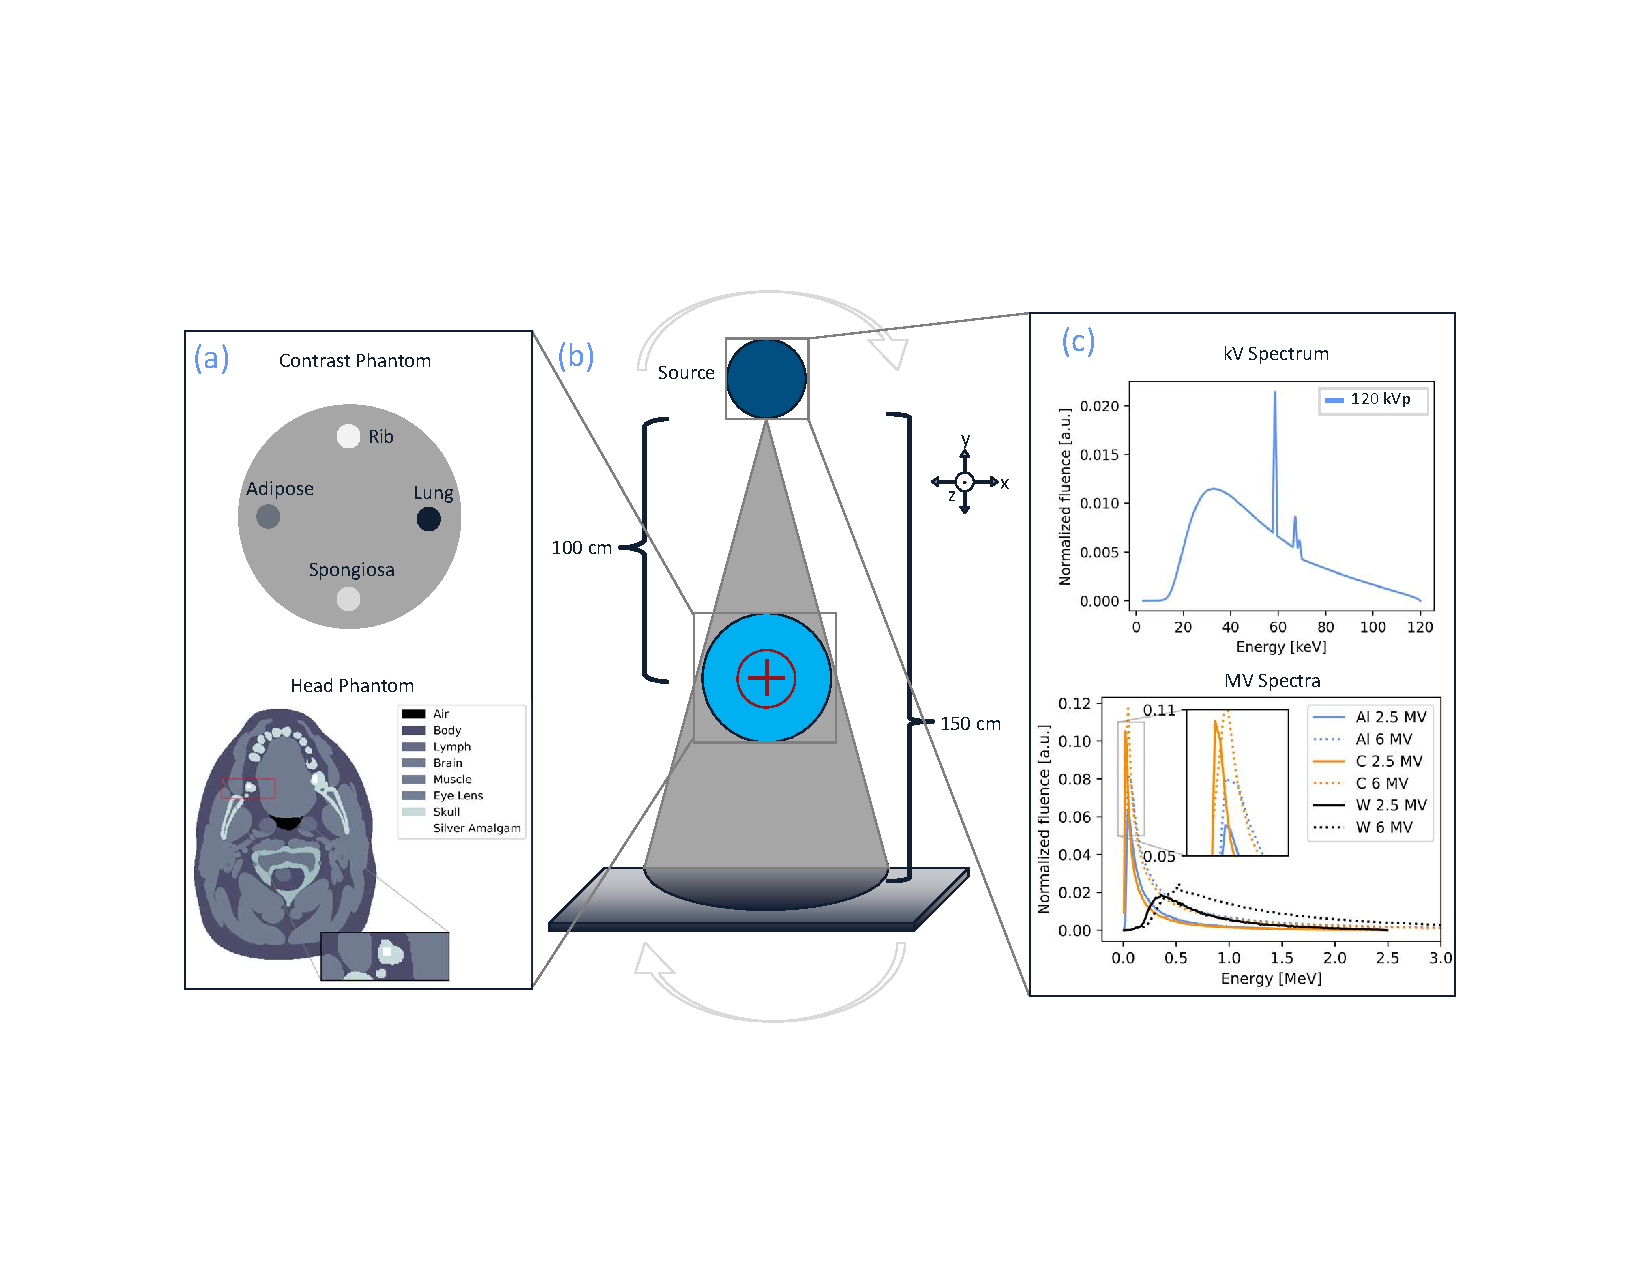
\includegraphics[width=0.9\linewidth]{figures/Figure_1.pdf}}
  \caption{The MTF of the CWO (a), CsI (b), and GOS (c) detectors as a function of the 120 kVp beam and the 2.5 MV and 6 MV carbon and tungsten target beams. MTFs were calculated from the presampled line spread function of an angled slit. Experimental MTF calculated by Shi \textit{et al.} \cite{Shi2019ADetectors.} for the GOS detector at 6 MV tungsten target beam is displayed in (c) which uses the angled slit MTF calculation method off of which all other measurements are based.
    }  %note label inside caption
    \label{fig_mtf}
    \centering
\end{figure*}

The MTF for the three detectors is presented in Figure \ref{fig_mtf}.  In all cases the 120 kVp beam resulted in the highest MTF at all spatial frequencies for a given detector. Likewise, in nearly all cases the highest energy beam, the 6 MV tungsten target resulted in the lowest MTF. For MV beams the CsI detector had the highest MTF compared to the other detectors. For the kV beam the CWO detector resulted in the highest spatial resolution at low frequencies while the CsI detector resulted in better spatial resolution at high frequencies. The CWO spatial resolution dropped off due to the Nyquist frequency enforced by the detector septa which were only present in the CWO detector. Conversely, the CWO detector had the worst spatial resolution in all cases other than the 120 kVp beam, as mentioned above.

\begin{figure*}[ht!]
   \begin{center}
%   \captionsetup{justification=centering}
   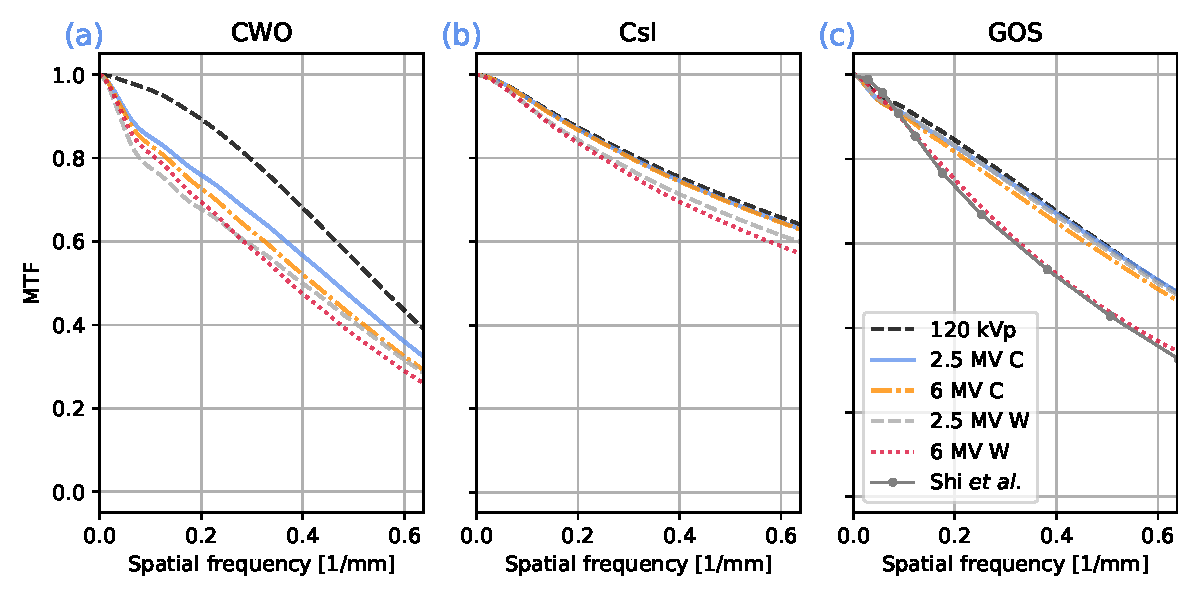
\includegraphics[width=0.9\linewidth]{figures/Figure_2.pdf}
  \caption{Simulated CBCT images of the contrast phantom reconstructed with the CWO (a,d), CsI (b,e) and GOS (c,f) detectors for the 120 kVp (a-c) and 2.5 MV carbon (d-f) beams (W/L 800/0 for images). All images were reconstructed using the FDK algorithm from 360 views with an imaging dose of 7 mGy. The inset shows the spongiosa insert.
   \label{fig_phan} 
    }  %note label inside caption
    \end{center}
\end{figure*}

\subsubsection{Contrast}

\begin{figure*}[h!]   
    \begin{center}
    % \captionsetup{justification=centering}
%   \begin{center}
    \centerline{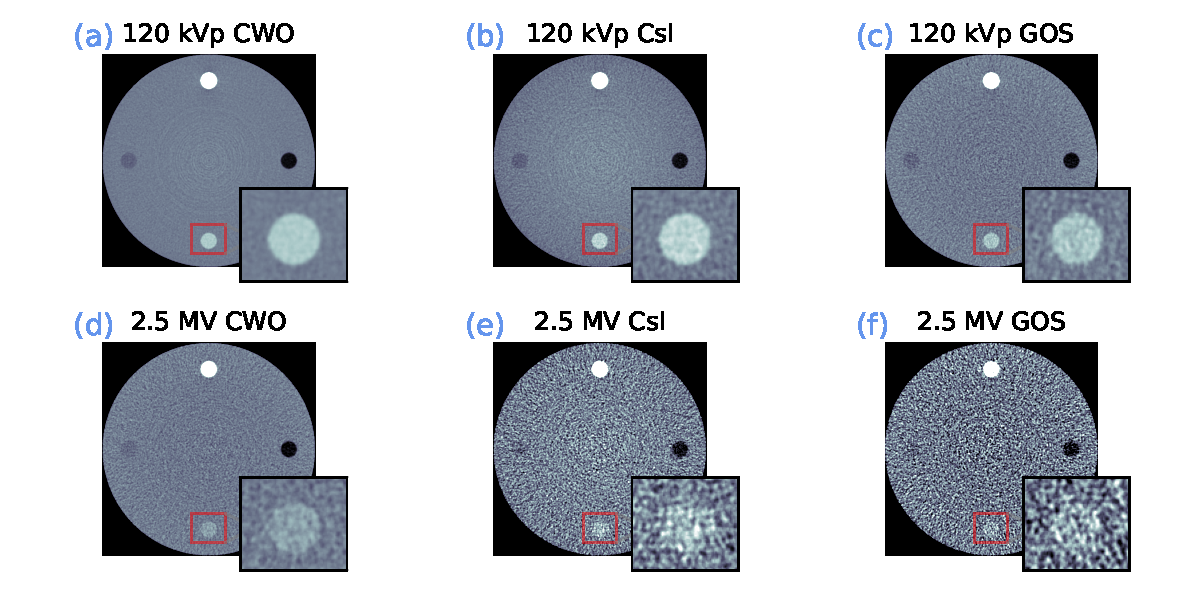
\includegraphics[width=0.9\linewidth]{figures/Figure_3.pdf}}

  \caption{The contrast to noise ratio for rib bone, lung, adipose and spongiosa tissues as a function of CWO (a), CsI (b), and GOS (c) detectors for different beam energies and a phantom dose of 7 mGy. \label{fig_cnr}
    }  %note label inside caption
    \end{center}
\end{figure*}
% For the 120 kVp beam the \# generally had the highest contrast with (Figure \ref{}) \#, \#, \#, and \# for the rib and spongiosa bone, adipose, and lung, respectively in terms of contrast. For the 2.5 and 6 MV carbon targets the \# had the best contrast with \#, \#, \#, and \# for the four materials, respectively. For the 2.5 and 6 MV tungsten targets the \# had the best contrast with \#, \#, \#, and \# for the four materials, respectively.

Some sample contrast phantom CBCTs are shown in Figure \ref{fig_phan} while CNR results for rib bone, lung, adipose, and spongiosa derived from CBCT images of the contrast phantom for the 120 kVp beam, the 2.5 MV and 6 MV beams with carbon and tungsten target and all three detectors are shown in Figure \ref{fig_cnr}.
CNRs for all materials were seen to decrease with average beam energy for all detectors. The highest CNRs were for the CWO detector with the 120 kVp beam; CNRs were 53.1, 47.9, 10.2, and 21.1 for the rib bone, lung, adipose, and spongiosa, respectively. CNRs for the CWO detector and carbon 2.5 MV beam were 28.1, 20.2, 3.6, and 2.5 for the rib bone, lung, adipose, and spongiosa, respectively. For the CsI and GOS detectors the 120 kVp beam produced the highest CNR over all inserts. The CNRs for the 120 kVp GOS were 27.2, 17.8, 6.6, and 3.4 for the rib bone, lung, adipose, and spongiosa, respectively. The CNRs for the  CsI detector and 120 kVp beam were 33.9, 22.2, 6.2, and 11.0 for the rib bone, lung, adipose, and spongiosa, respectively. Finally, the highest-energy 6 MV tungsten target showed the lowest CNR for each detector.

\subsubsection{Head phantom CBCT imaging}


CBCT images of the head phantom with silver amalgam fillings for two beam energies and all three detectors are presented in Figure \ref{fig_xcats}. The CBCT images are in agreement with CNR results. Qualitatively, the 120 kVp image shows good contrast as well for both the CWO and CsI detectors (Figure \ref{fig_xcats} a, b). Increased noise becomes prevalent in the images acquired with the CsI and GOS detectors (Figure \ref{fig_xcats} e, c, f). Streaking artifacts are most prevalent in the 120 kVp images, obscuring much of the soft tissue. Likewise, the 2.5 MV images with CsI and GOS detectors show increased streaking artifacts as compared to the CWO image which shows the best preservation of tissue contrast in the soft tissue surrounding the inserts.

\begin{figure*}[ht!]
   \begin{center}
%   \captionsetup{justification=centering}
   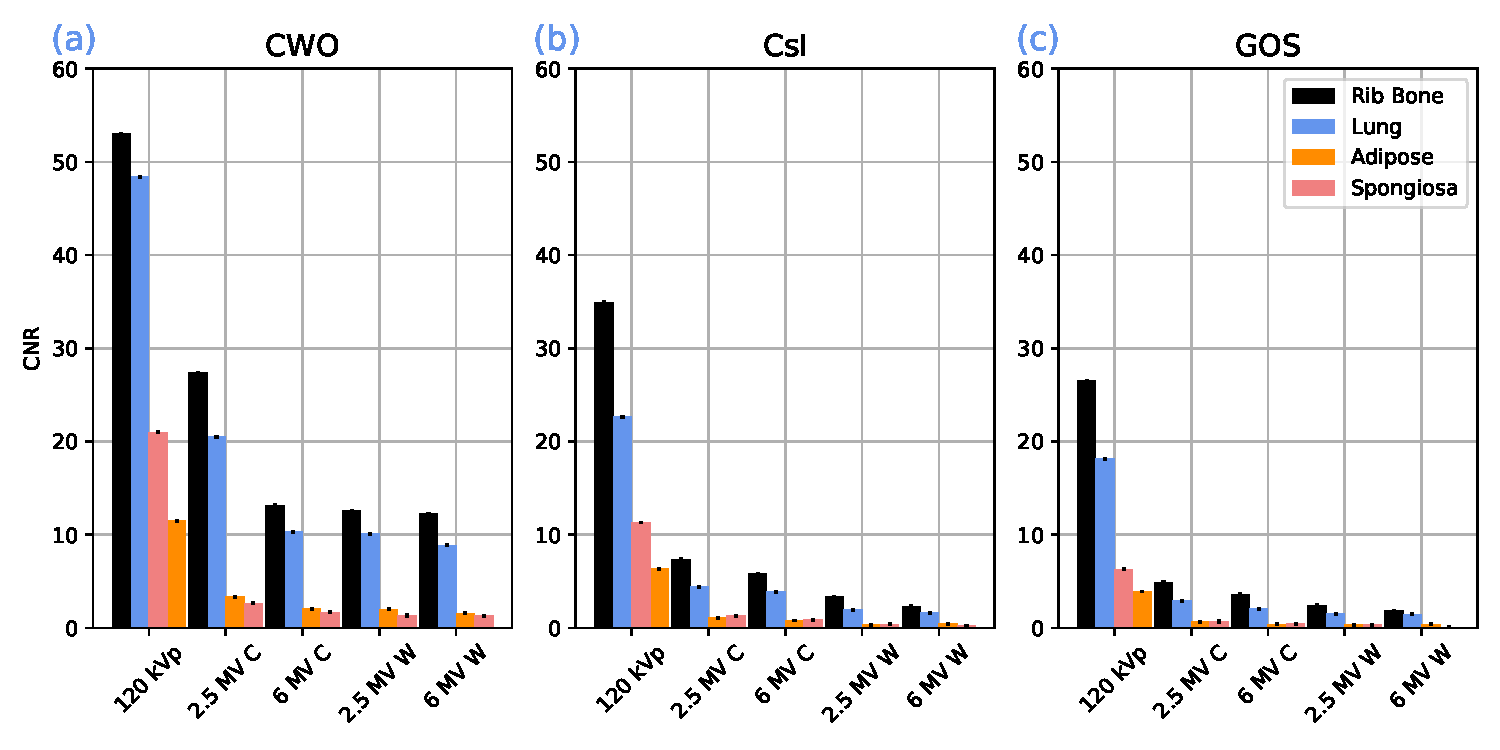
\includegraphics[width=0.9\linewidth]{figures/Figure_4.pdf}
  \caption{Simulated CBCT images of an XCAT head phantom with silver amalgam fillings reconstructed with the CWO (a,d), CsI (b,e) and GOS (c,f) detectors for the 120 kVp (a-c) and 2.5 MV carbon (d-f) beams (W/L 800/0 for images and 1100/450 for inset). All images were reconstructed using the FDK algorithm from 360 views with an imaging dose of 7 mGy.
   \label{fig_xcats} 
    }  %note label inside caption
    \end{center}
\end{figure*}

\subsection{Discussion}

The results of the CNR study presented in Figure \ref{fig_cnr} demonstrate a promising MV beam/detector combination. Undoubtedly, the CWO 120 kVp results in the largest CNRs. However, the CWO CBCT images acquired with the 2.5 MV beam resulted in CNRs comparable to the 120 kVp beam with a CsI or GOS detector. Additionally, this combination shows promise in suppressing metal artifacts, as seen in Figure \ref{fig_xcats}. This improvement is in part due to the increased dose efficiency at higher energies, as well as the high absorption efficiency of the CWO relative to the GOS and CsI at MV energies. If high contrast images could be acquired using an EPID, linear accelerator design could be streamlined in some cases by removing the OBI, which would in turn result in reduced linear accelerator costs.

Conversely there are some downsides to this combination. The MTF for the CWO detector with the 2.5 MV carbon target is lower compared to that of the GOS and CsI detectors at all spatial frequencies. The CWO spatial resolution performed differently as a function of beam energy, due to the CWO detector septa. CWO exhibits low attenuation of optical photons at its scintillation energy, resulting in the need for pixel septa to funnel the photons towards the amorphous silicon readout. These septa resulted in a very good MTF at low energies where relatively few interactions in the detector pixel resulted in secondary particles crossing the detector septa and causing scintillation in other pixels. At higher energies the septa were often breached by secondary particles leading to a wider point spread function. However, with the beams discussed, secondary particles did not manage to breach the septa of the adjacent pixels (breaching two septa in total) in large quantities. This led to the two groupings of MTF curves in the CWO detector; a high resolution curve for the 120 kVp beam and the low resolution curve for the rest of the beams. The CWO and GOS detectors showed slowly decreasing MTFs as a function of beam energy with the CsI detector performing slightly better due to its columnar structure. Thus, the CWO detector, at least with the pixel size discussed, shows a disadvantage in terms of spatial resolution as compared to CsI and GOS detectors especially for spatial frequencies above the pixel pitch.

% Some of the characteristics of real imaging systems were intentionally excluded from simulations in this work. While Fastcat demonstrates the ability to accurately model certain commercial flattening filters for MV imaging and bowtie filters and anti-scatter grids for kV imaging \cite{OConnell2021ExperimentalSimulator}, these models were not used in an effort to maintain a fair comparison between beam/detector combinations. The flattening filter was excluded in favour of an idealized uniform beam as the flattening filter is designed for therapy applications and results in cupping artifacts. Likewise, the bowtie filters and anti-scatter grid were excluded in the kV CBCT simulation. We acknowledge that these additional features could led to different results of kV CBCT CNR calculations. These design features will be a topic of future work.

Additionally, the pixel pitch for the detectors was limited to 0.784 mm to model the dimensions of a current CWO detector design\cite{Star-Lack2015AImaging}. The ability to make smaller pixels of CWO in order to achieve high pixel uniformity is a current limitation of this detector\cite{Lindsay2019InvestigationDetector}. This limitation is not shared by the GOS and CsI detectors which are commonly produced with smaller pixel sizes defined by their amorphous silicon readout, since they do not require septa. Further, pixel uniformity is generally easily achievable with GOS and CsI detectors, while it is more challenging in CWO detectors. CsI and GOS detectors models examined in this work followed design specifications of existing experimental systems optimized for kV CBCT and MV portal imaging, respectively.

One should note that some of the MTF curves in this publication have been previously validated against experimental beams in previous studies of fastcat \cite{OConnell2021FastCAT:Simulation,OConnell2021ExperimentalSimulator}. Specifically, the 6 MV MTF curves for the CWO and GOS detectors were compared to experimental results from Star-lack \textit{et al.} and Shi \textit{et al.}, respectively \cite{Star-Lack2015AImaging,Shi2018APerformance}. With MTF values found to have an average root mean squared error (RMSE) of 3.5\% and 1.2\% compared to experimental values for the CWO and GOS detector respectively. Fastcat's experimental MTF curve was also validated against an experimental beam using the measurements of Howansky \textit{et al.} \cite{Howansky2017DirectImaging} with results within 4.2\% of measurements. In terms of CNR results, kV and MV CNR values were compared between a fastcat simulation of a Catphan CTP404 phantom and an experimental CBCT volume acquired using the OBI and EPID of a Varian Truebeam STx linac.

One question that arises with the use of low-Z target beams is the reduced bremsstrahlung yield compared to high-Z target beams which may affect the length of the image acquisition. There is experimental evidence to suggest that sufficient fluence would be generated, previous studies have shown photon yields from low-Z beams high enough for normal CBCT acquisition at energies above 1.9 MeV \cite{Parsons2012BeamTargets}. Additionally, there is a trade-off between having a small focal spot size for optimal spatial resolution and acquisition time. Linac focal spot sizes are generally larger than the ones of x-ray tubes. However, on the Truebeam OBI the large kV x-ray tube focal spot size is quoted as 1.0-1.4 mm by 1.4-2.0 mm while the linac electron beam has a focal spot size of approximtely 1.5 mm \cite{Lopez-Sanchez2019AnParameters}. This focal spot size could be improved by moving the target higher in the linac head where the electron beam is less divergent or including additional collimation at the target to decrease the focal spot size. However, in previous work by Chan \textit{et al.} MV CBCT system MTF, as determined using the Catphan CTP 528 module, was seen to be worse than that of kV CBCT \cite{Chan2011EvaluationSystems}. Contributing factors to this poor MTF were the decreased contrast of acrylic in the MV range as well as larger focal spots for some MV CBCT setups and the inherent decrease in detector MTF due to the larger MV point spread function as seen in this work.

The demonstration of the increased contrast in the XCAT head phantom CBCT images with the CWO detector and the carbon 2.5 MV beam is compelling as this shows better soft tissue resolution surrounding the silver amalgam fillings compared to the other beam/detector combinations discussed (Figure \ref{fig_xcats}d). This demonstrates the possibility of using this beam in some treatment sites for the benefit of metal artifact reduction.


% \subsection{Conclusion}

% Novel kV/MV CBCT beam/detector combinations were simulated using low-Z beam target spectra and three x-ray detectors. CNR was highest in the CWO detector with a 120 kVp beam. The 2.5 MV carbon target beam combined with a CWO detector showed CNR 4\% and 17\% lower than current CsI/120 kVp kV imaging systems in lung and bone, respectively and performed best at metal artifact reduction in the XCAT phantom. Whereas, the detector MTF was seen to be highest for a kV beam with the CWO detector at low frequencies, GOS and CsI were seen to outperform CWO in terms of MTF for all MV beams and at high frequencies for the kV beam.

% \subsection{Acknowledgements}

% This research was enabled in part by support provided by WestGrid (www.westgrid.ca) and Compute Canada Calcul Canada (www.computecanada.ca). The work was partly funded by an NSERC Discovery Grant and the Canada Research Chairs program. 